\section{The Problem}

The Wikipedia's continued success depends on ill-intentioned users
not being able to overwhelm the well-intentioned users.
Communities are complicated systems, with people constantly joining and
leaving their membership.
We can suppose that people continue to
join the Wikipedia community because most pages are
substantially useful, and users feel that their contributions
\textit{add} to the resource,
giving them a sense of satisfaction~\cite{Benkler2002}.
If the amount of vandalism occurring were to increase so that
most users were only \textit{repairing} the Wikipedia, there
would be much less satisfaction.

The key problem this community faces is in quickly identifying vandalism
to prevent the appearance (to casual users)
of needing maintenance.
The RC Patrol~\cite{wiki:RCPatrol} acts as a guardian,
investing a large amount of human capital to scan all
edits made to the Wikipedia, searching for vandalism and
other inappropriate edits.
Still, it is possible to sneak vandalism by the
RC Patrol; the article on \underline{South Pasadena, California}
was vandalized in May~2008 to include a Nazi propaganda film,
which persisted until April~2009.\footnote{See Chapter~\ref{ch:editquality}
for more details.}

\begin{figure}[t]
\centering
\subfloat[
  coloring of an article before vandalism][
  Before the modification~\cite{wiki:Denmark-Fogh}.]{
  \label{fig-denmark-a}
  \framebox{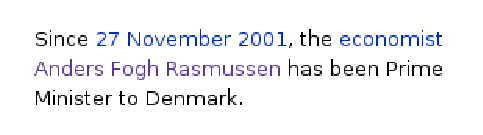
\includegraphics[width=0.45\textwidth]{part-C10-intro/Denmark-Fogh}}
}
\hspace{1ex}
\subfloat[
  coloring of an article after vandalism][
  Immediately after the modification~\cite{wiki:Denmark-Fjogh}.]{
  \label{fig-denmark-b}
  \framebox{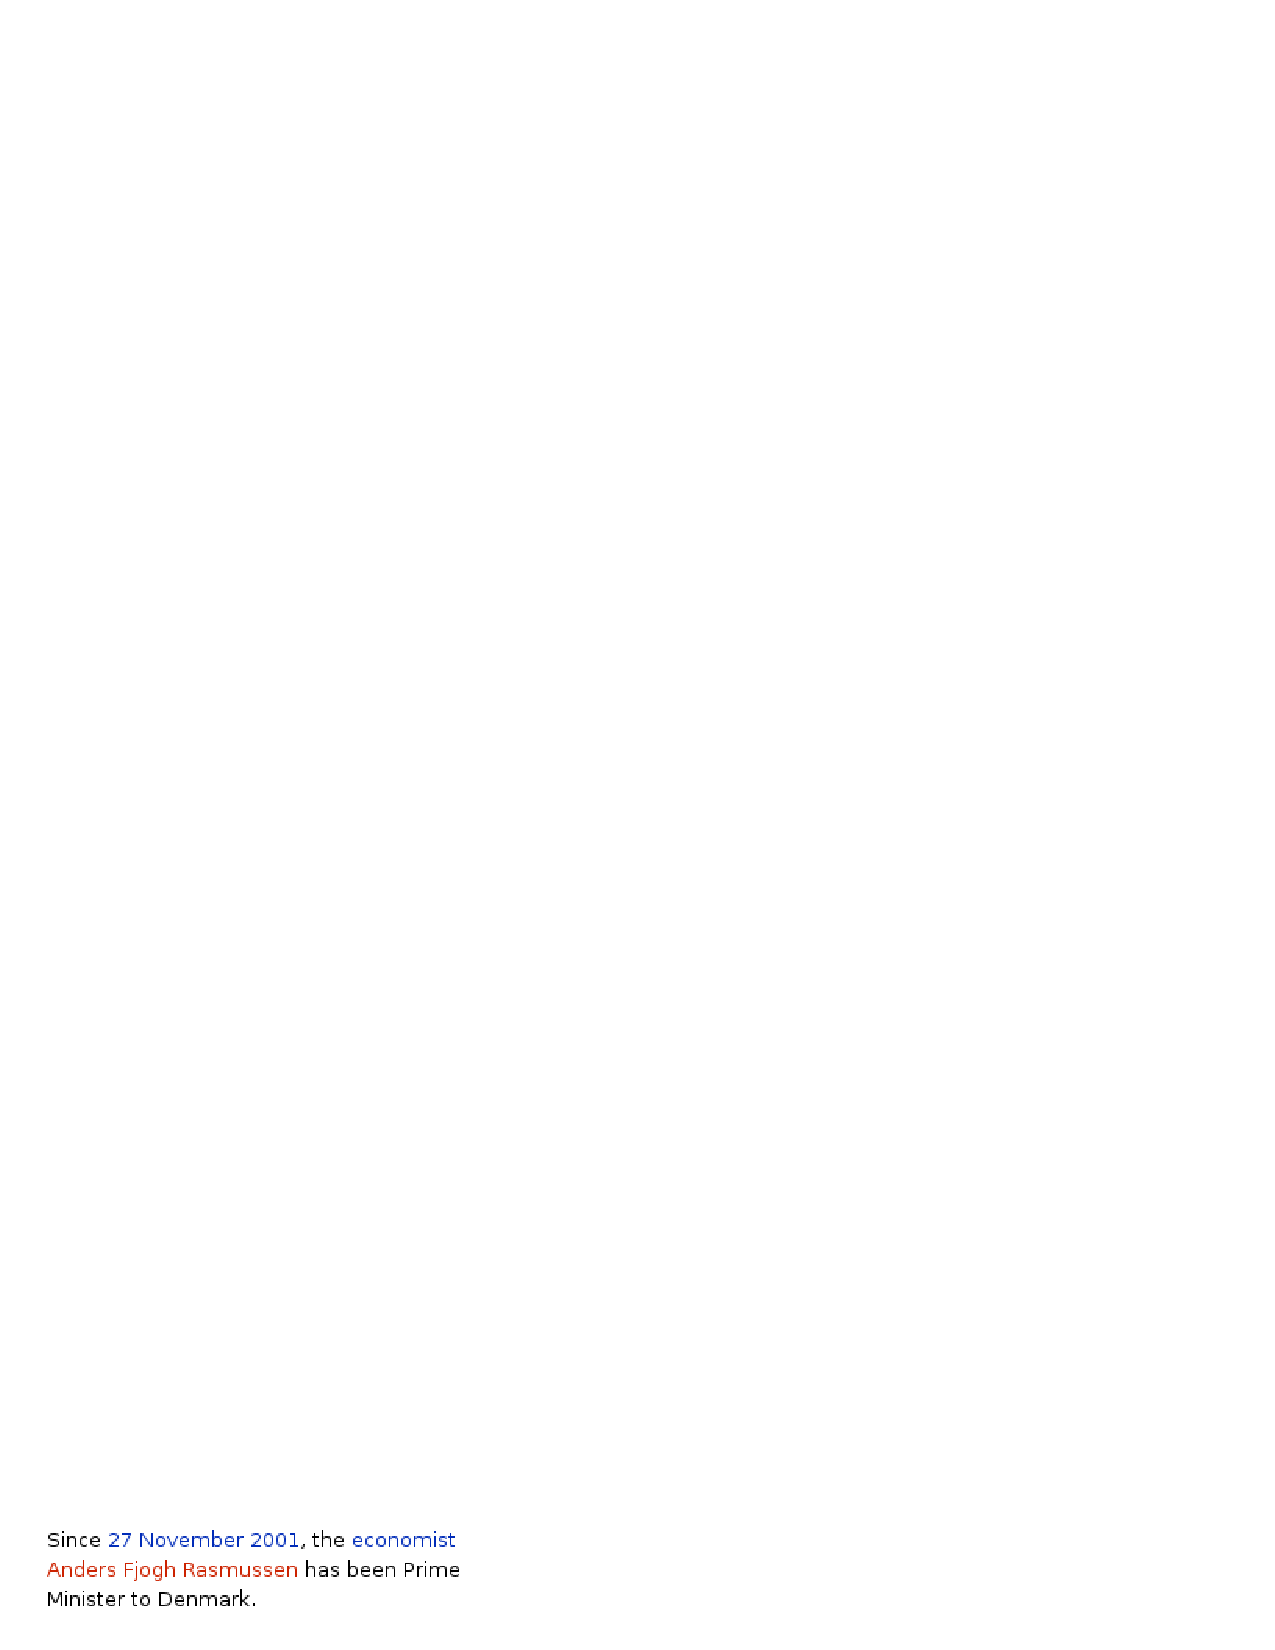
\includegraphics[width=0.45\textwidth]{part-C10-intro/Denmark-Fjogh}}
}
\caption[An example of vandalism which is not obvious to the casual reader]{
  An attempt to modify the
  spelling of the Danish Prime Minister's last name, from Fogh to Fjogh.
  The casual user, who does not speak Danish and happens to check
  the version history, has little indication on which might be correct.
  This is a case of vandalism
  (in Danish, a \textit{fjog} is a \textit{fool})
  that is quite subtle and most users would not even notice.}
\label{fig-denmark}
\end{figure}


Vandalism can be very hard to identify for inexperienced users.
Consider the example of Figure~\ref{fig-denmark},
which is an excerpt from the \underline{Politics of Denmark}
entry in the English Wikipedia: an anonymous user substitutes
``Fjogh'' for ``Fogh'' in the Prime Minister's last name.
This is a particularly subtle kind of vandalism,
because it requires knowledge of Danish
(\textit{fjog} translates to \textit{fool} or \textit{goofy})
to recognize this change as anything more than a spelling correction.
A sophisticated reader might recognize the broken link
as a hint on the true spelling, or even try to use Google
to research the name (both spellings return results, however).
The level of effort to recognize the error and to
verify this relatively small detail is quite high.

Beyond vandalism, another issue that affects the perceived
quality of the Wikipedia are well-intentioned users that contribute
very low-quality material.
For instance, material written from a
neutral point of view\footnote{\url{http://en.wikipedia.org/wiki/Wikipedia:Neutral_point_of_view}}
promotes the Wikipedia as an impartial resource that welcomes contributions
from all parties.
When a contribution does not adhere to this standard, the bias
detracts from the credibility of the article and can discourage
other users from participating in the community.

Historically, there are three inter-related approaches to
attaching value to knowledge.
The most familiar method is \intro{formal publication} by an organization
that stakes their reputation on the material;
the Encyclop{\ae}dia Britannica is one famous example.
To achieve their high quality, experts write the articles in the
Encyclop{\ae}dia Britannica
and then peers and an editorial staff review them.
\intro{Peer review} is a second approach to the creation of
knowledge; science extensively uses this method,
but we distinguish it from ``formal publication'' because
only the actual authors stand behind the veracity of the
material being reported.
\intro{Reputation} is a third approach attaching value
to knowledge; people naturally ascribe reputations to other
individuals and will accept knowledge without verification from
sources that they feel have a high enough reputation.

The overarching question for the Wikipedia is
\textit{how do we maintain the good quality of articles?}
The historical approaches have all translated to online
knowledge repositories (\eg Google Knol\footnote{\url{http://knol.google.com}}
and Encyclop{\ae}dia Britannica
are based on formal publication,
Nupedia~\cite{wiki:Nupedia}
was based on peer-review,
and Stack Exchange\footnote{\url{http://stackexchange.com}}
implements an explicit reputation system).
We propose that constructing an automated reputation system
for the Wikipedia would facilitate the detection of vandalism.

